\documentclass[12pt]{article}

\usepackage[paper=letterpaper,margin=2.5cm]{geometry} % Set Margins

%% Math and math fonts
\usepackage{amsmath, amsthm, amssymb, amsfonts}
\usepackage{bbold} % for \mathbbm{1}

% date
\usepackage[nodayofweek]{datetime}

% Color
\usepackage{color, xcolor}

% Misc
\usepackage{environ}  % \collect@body in asmmath
\usepackage{graphicx} % \includegraphics options
\usepackage{mdframed} % text boxes
\usepackage{indentfirst} % Indent first paragraph after section header
\usepackage[shortlabels]{enumitem} % Control enumerate items with [(a)]
\usepackage{comment} % Comments
\usepackage{fancyhdr} % Headers and footers
\setlength{\headheight}{14.5pt} % Fix fancyhdr warning

% Tables
\usepackage{array}

% Sub-figures and figure placement
\usepackage{caption}
\usepackage{subcaption}
\usepackage{float} 

% Graphing
\usepackage{pgfplots}
\pgfplotsset{compat=1.17}
\usepackage{tikz}

% Title Placement
\usepackage{titling}
\setlength{\droptitle}{-6em}

%set indent to 
\setlength{\parindent}{0pt}
\setlength{\parskip}{10pt}

% Hyper refs
\usepackage{hyperref}
\hypersetup{
    colorlinks=true,
    linkcolor=blue,
    urlcolor  = blue,
    filecolor=magenta,      
    urlcolor=blue,
    citecolor = blue,
    anchorcolor = blue
}

% % Citation management
\usepackage{natbib}
\bibliographystyle{abbrvnat}
\setcitestyle{authordate,open={(},close={)}}

% ----------------------------------------
% TITLE
% ----------------------------------------

\pagestyle{fancy}

\lhead{Camacho}
\chead{Class 2}
\rhead{FAME}

\title{FAME Class 2 Notes -- Mathematics as Creative Symbolic Reasoning}
\author{Mariana Camacho}

\begin{document}
\maketitle

\section{Review from last class}
\subsection{Sets and domains}
\(x\in X \in \mathbb{R} \)\ means that there is some value of x in the set of all possible X values. We can think of this as the sizes of a mature tree, values between 7 and 35 feet (this is the domain). Everything within 7 and 35 feet is within the set of real numbers. 

It is also possible for x to be restricted to the natural numbers: \(x\in X \in \mathbb{N} \). The type of number depends on the question that we're thinking about. 

\subsection{Question from video}

We can write 
\(rx-\alpha rx^2=0\)\ as \(rx(1-\alpha x)=0\)\, and define: \(a=rx\)\ \& \(b=1-\alpha x\)\ . One of the two terms or both have to be zero in order for the value of the function to be zero. This equation might represent us trying to figure out when something is not changing. 

\subsection{Logs and exponents}
There are two common notations for exponents: \(e^x\)\ and \(exp(x)\). Some people switch back and forth, but these are exactly the same thing. 

\subsubsection{Definition of e}

As you will see in the book, the formal definition of e is:
\(e^{- \pi \mathrm{i}}-1=0\)\ (Fun fact: all math comes from 0,1, \(e\)\, \(\pi\)\ and the imaginary number \(\mathrm{i} \)\ ).

\subsection{Jensen's inequality}

The essence of Jensen's inequality is that when we have two non-linear relationships, we can't reverse them. Order of operations is a special case of Jensen's inequality.

This is challenging because humans really like lines. This is one of the most common mistakes made in scientific papers. 

This is a yellow flag - a point where we need to slow down and be extra careful. Knowing how to recognize these will be one of the key takeaways from this class. 

\section{Systems thinking}
Systems thinking got brought up a lot during the first half on the term. Now, we will think about what it means to be a systems thinker in the context of applied math. 

Last class, we talked about functional relationships, such as: \(y=f(x)\)\ . This equation is a simple system, that can be modeled in something like the plot below, which shows the relationship between rainfall and tree growth (it doesn't need to look exactly like this, it can also be a straight line or something completely different). 

\begin{figure}[H]
    \centering
    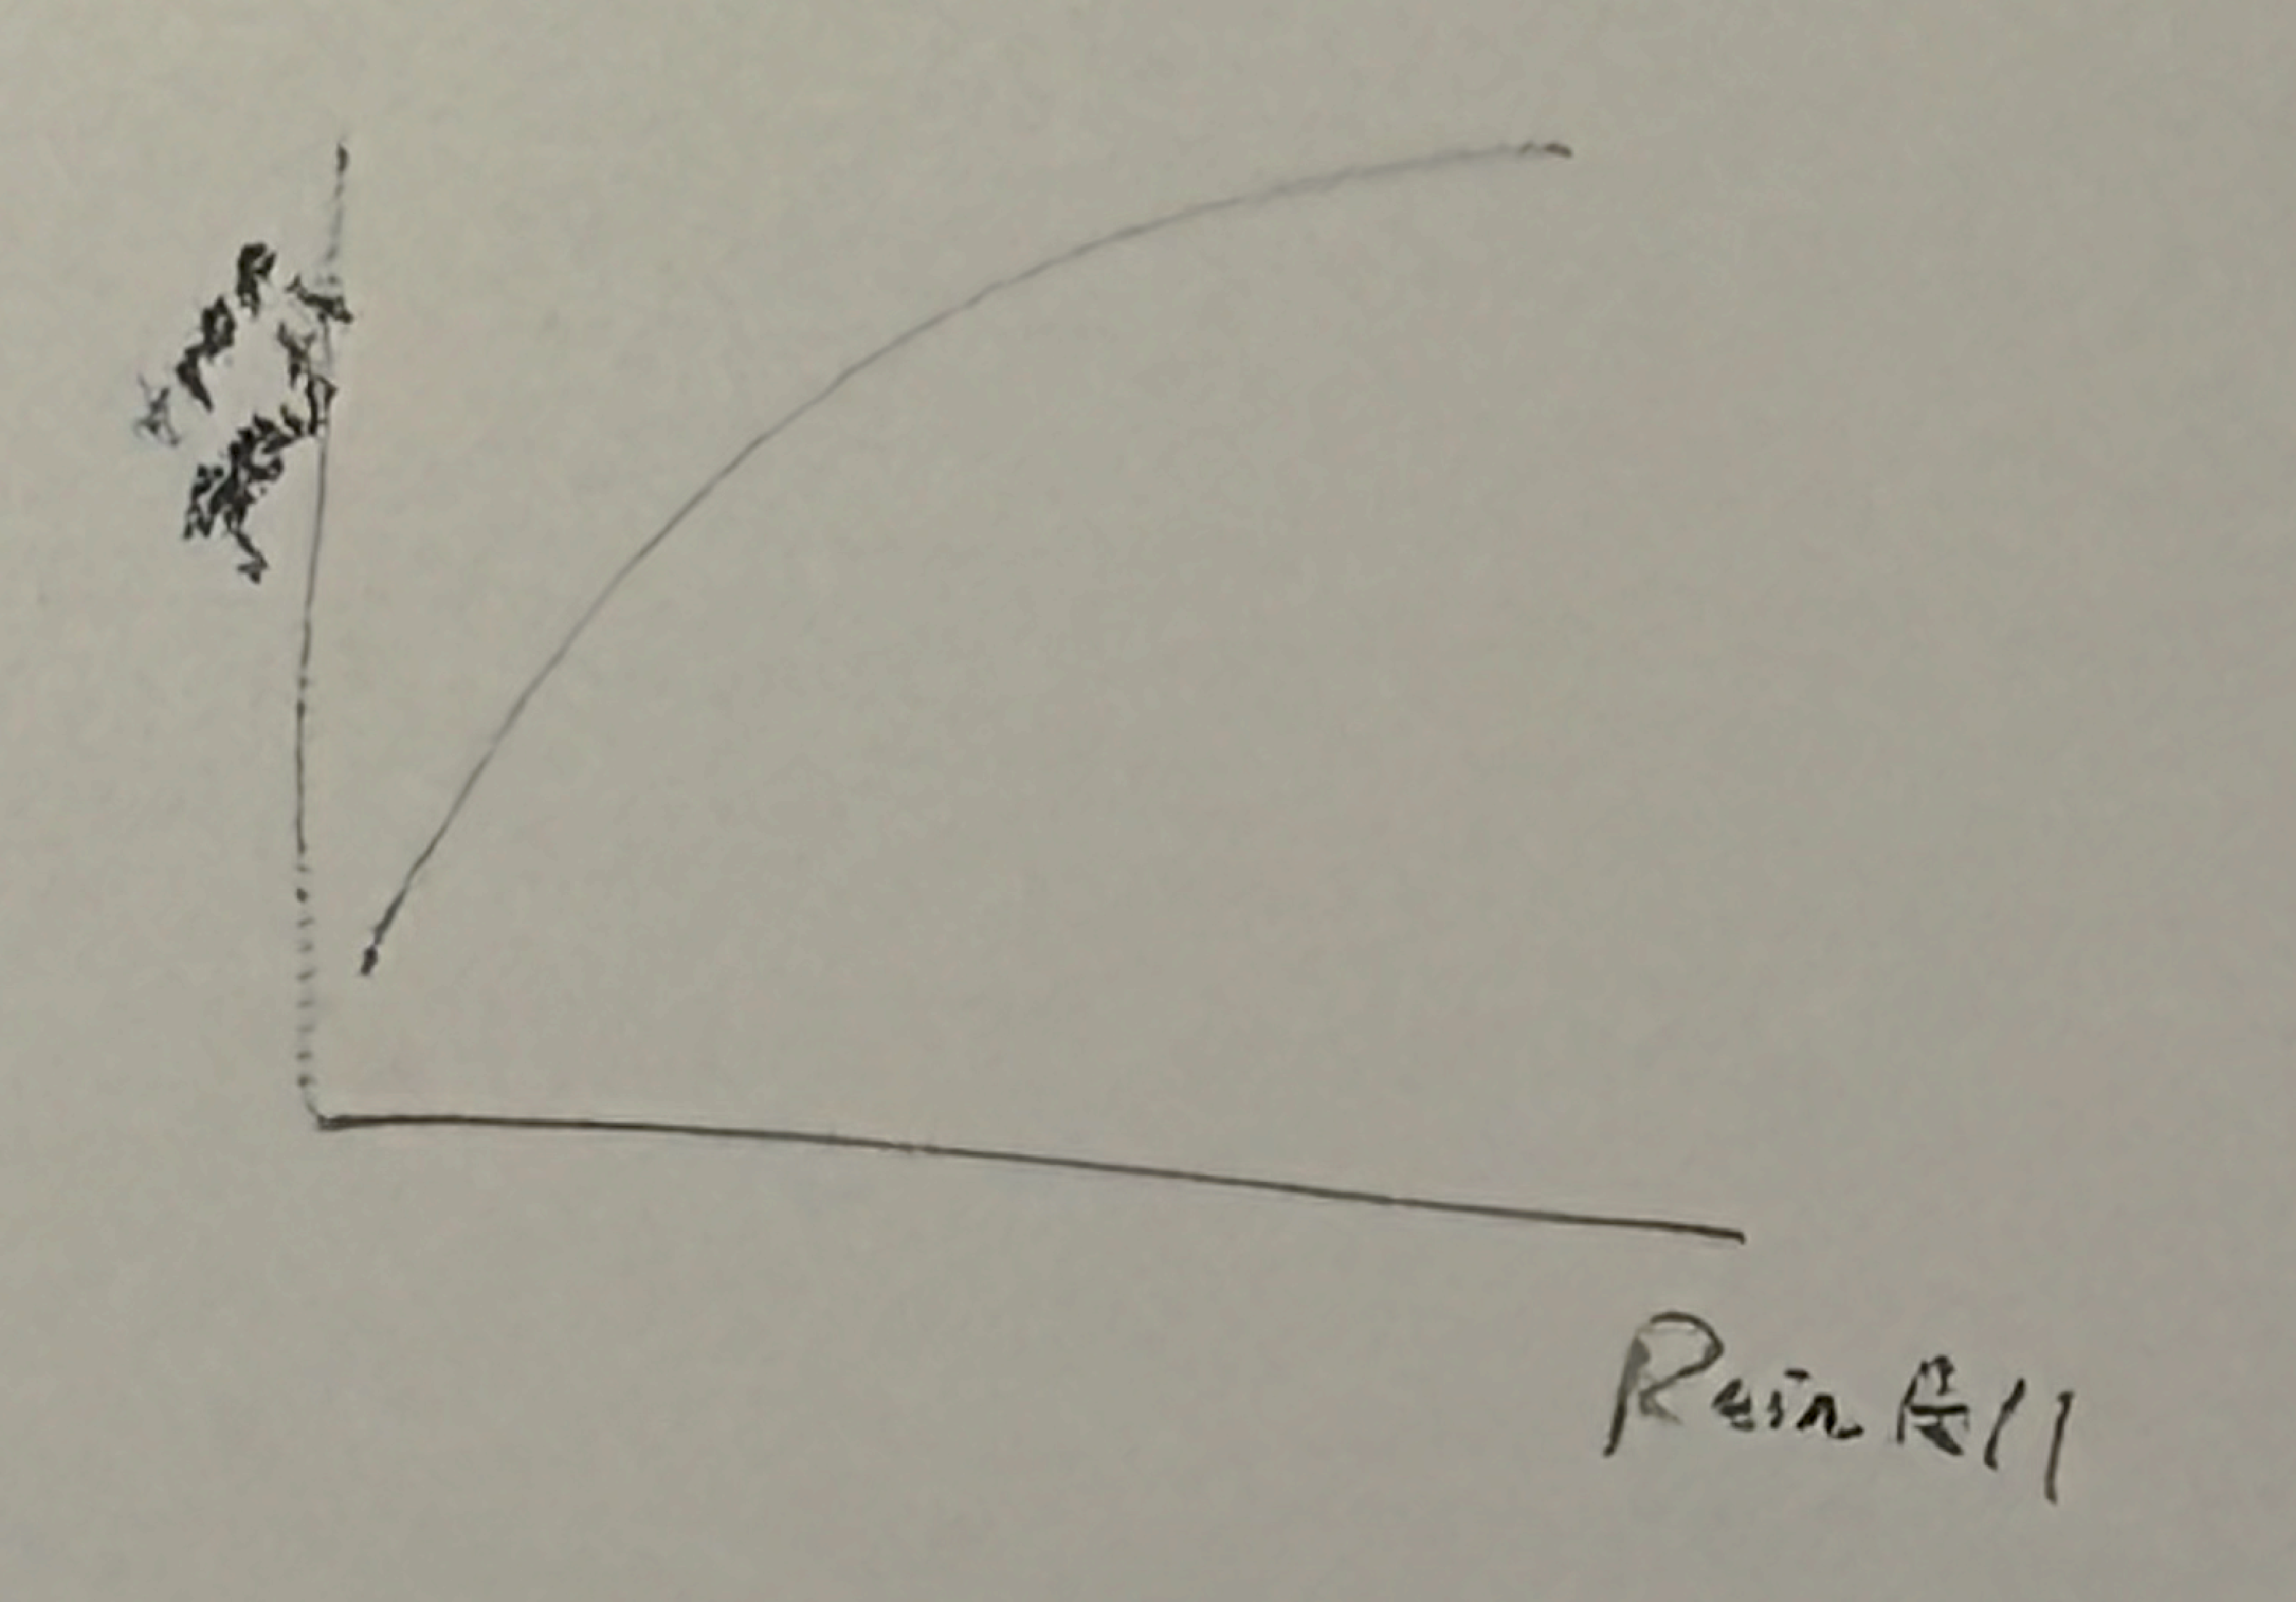
\includegraphics[width=0.5\linewidth]{class_notes/class_2/rainfall_plot.pdf}
    \label{fig:rainfall_plot}
\end{figure}
Let's assume that: \(f(x)=a+bx\)\

There might also be another relationship:
\(x=c-dy\)\ 

Once this comes in, we might start to have a system that looks like this.

\begin{figure}[H]
    \centering
    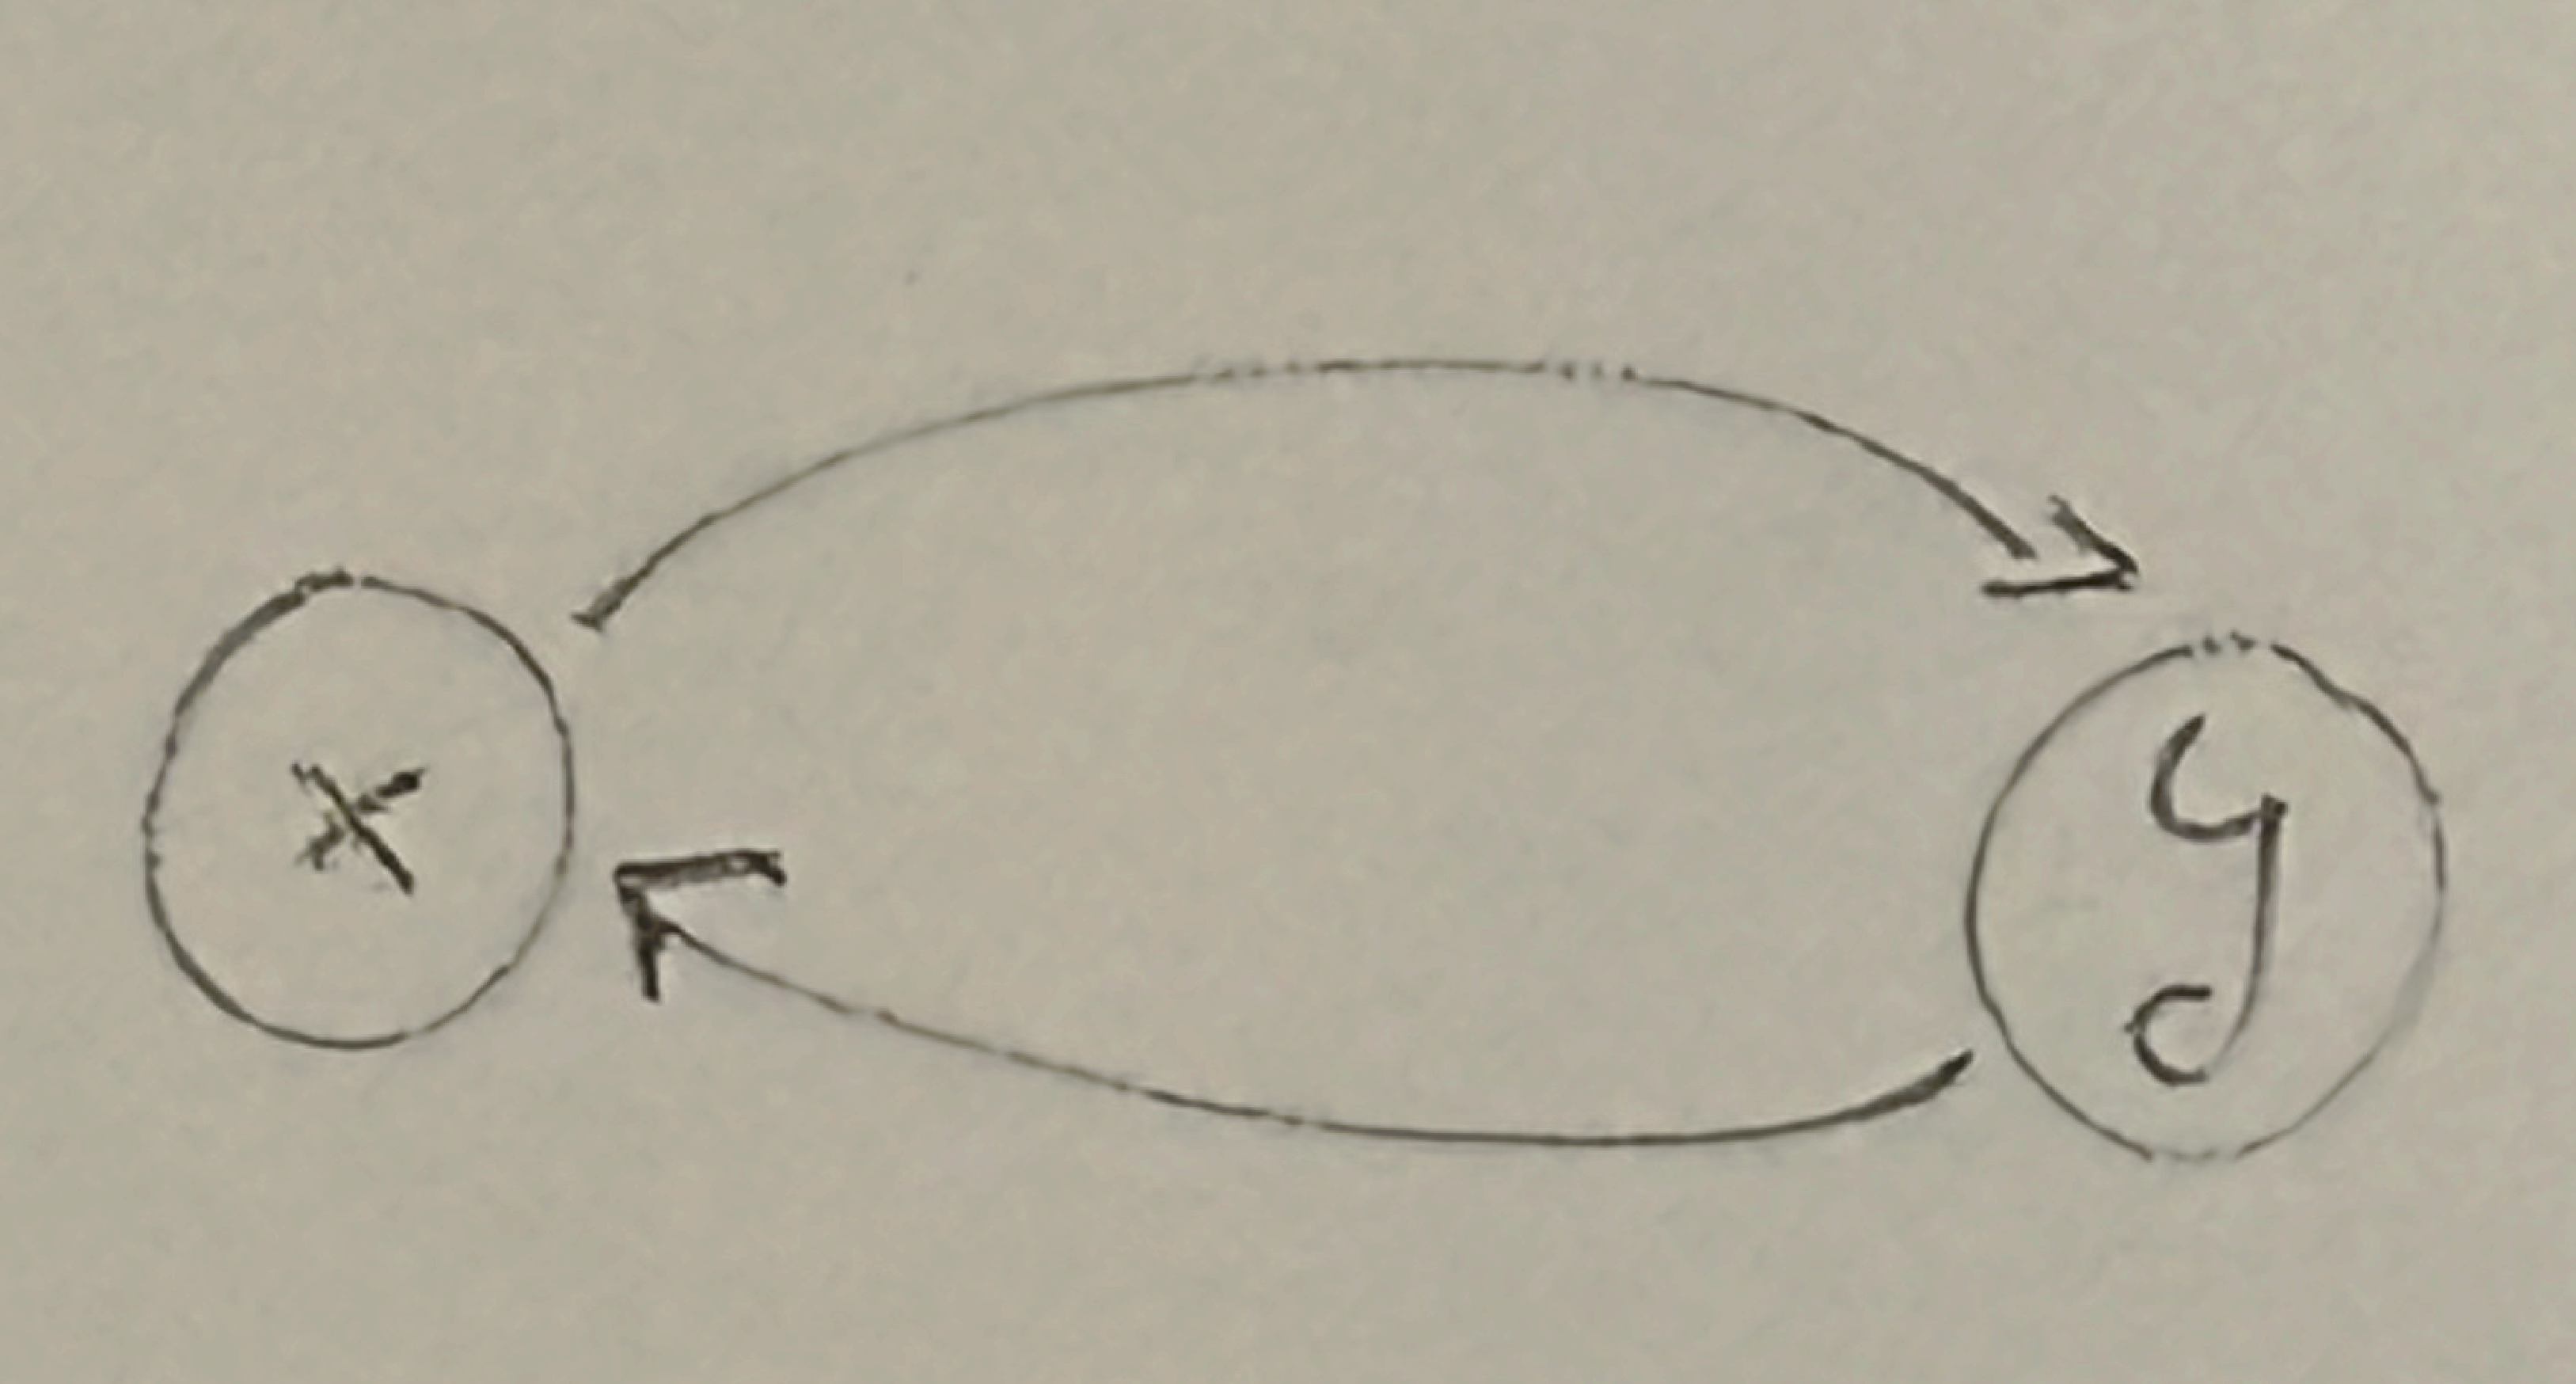
\includegraphics[width=0.25\linewidth]{class_notes/class_2/model_diagram.pdf}
    \label{fig:model_diagram}
\end{figure}

\textbf{Exogenous variables} are the things that we take as given. Often we're more interested in the \textbf{endogenous variables} (things in black circles), the variables that we model. With this, we can start drawing graphs and networks of relationships.

We can solve a system, and call that an \textbf{equilibrium}. An equilibrium is when multiple things are equal, or when things aren't changing (specific definition often depends on the field, and whether they're concerned about dynamic processes).

\subsection{Implicit functions}
We can write an implicit function as: \(G(x,y;a,b,c,d)\)

We can also write it as: \(G(x,y)\)

This means we can write a relationship between x and y, taking some things as given (in the equation above, we would take $a$, $b$, $c$ and $d$ as given).

\subsection{Small aside: the role of data}
In math, we have the opportunity to not start from the data, but start from defining relationships that we're interested in. In our field, we often want to model complex relationships, but we don't always have all the data to model it. 

\subsection{Systems of equations}
We tend to want to work with systems of equations (i.e. multiple equations that are solved simultaneously). For example:

\(ay+bz=u\)\\
\(cx+dz=w\)\\
\(fx+gy=v\)\\

We can think of these as linear equations. We will introduce some new notation to make this simpler - \textbf{matrices}!

\subsection{Matrix notation}
Matrices are just a notational shift, which allows us to use different tools. First, we want to line everything up neatly.

\(0x+ay+bz\)\\
\(cx+0y+dz\)\\
\(fx+gy+0z\)\\

We just used one of the two most common tricks in mathematics: adding zero. (Fun fact, the second one is multiplying by one). 

Now that our system looks nice and neat, we can rewrite it in matrix notation as shown below:

\begin{figure}[H]
    \centering
    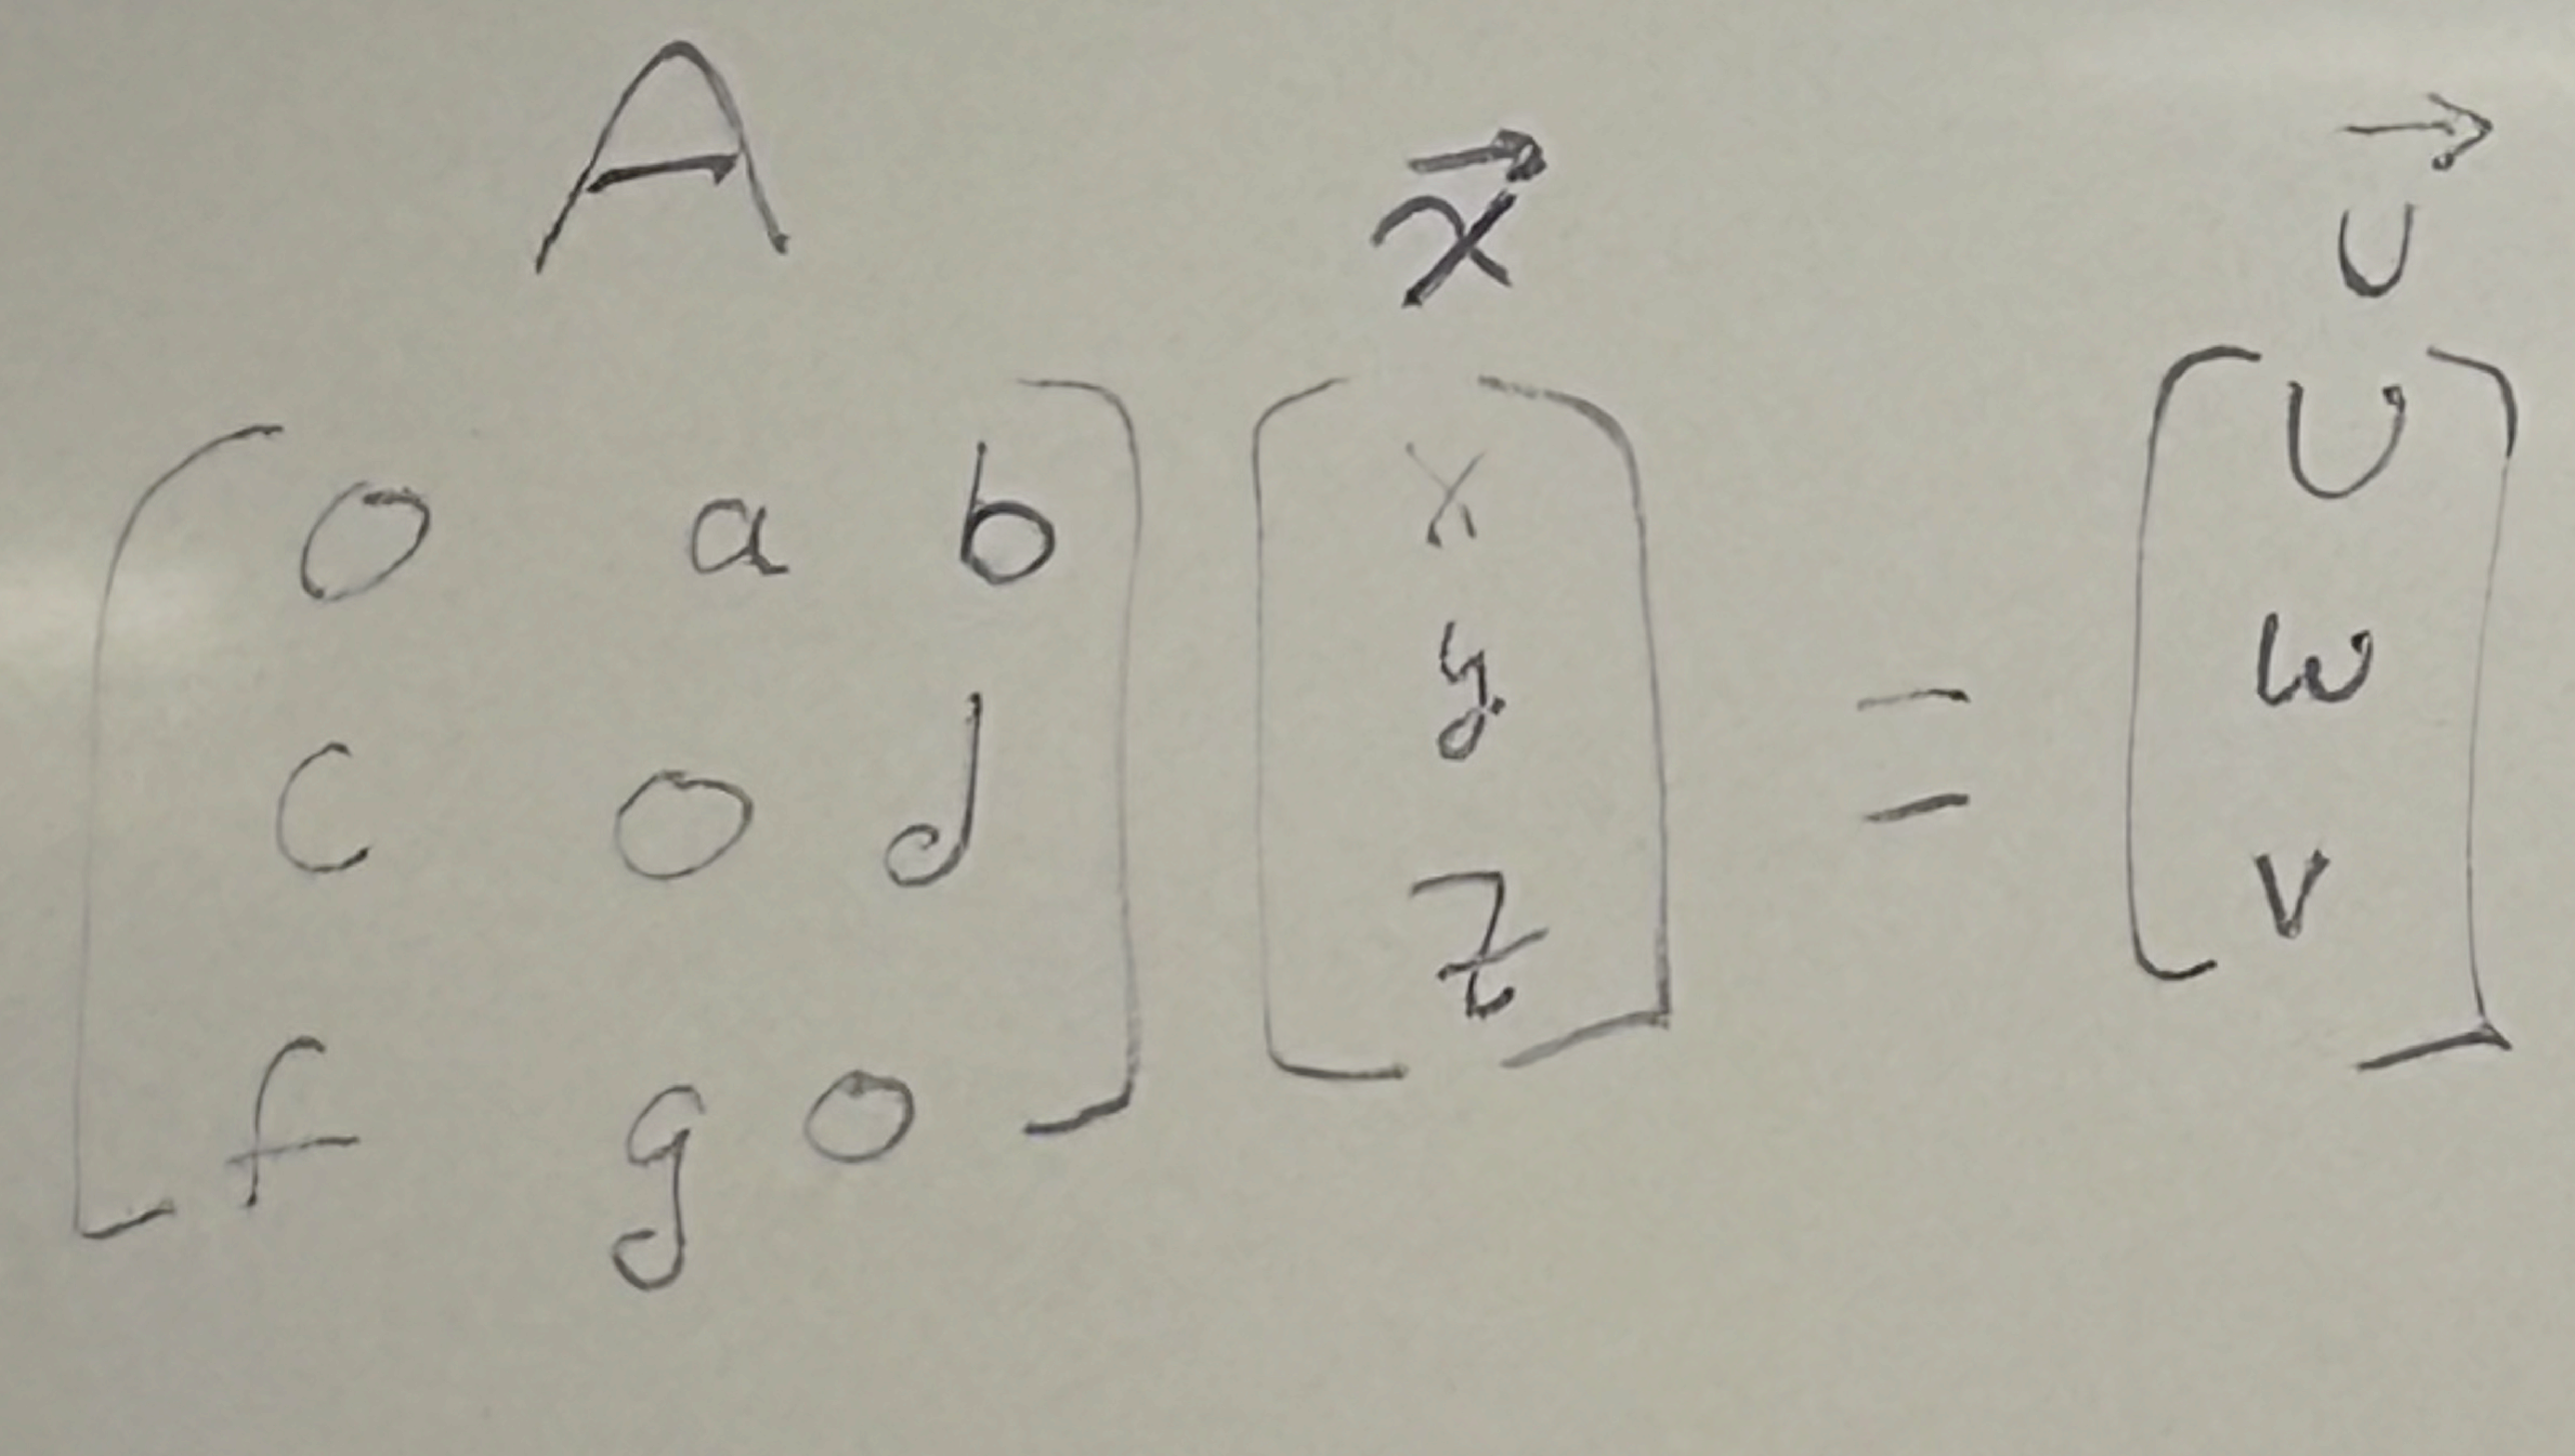
\includegraphics[width=0.5\linewidth]{class_notes/class_2/matrix_example.pdf}
    \label{fig:matrix_example}
\end{figure}

We haven't changed anything, we just reorganized the notation. This is helpful because now we can call the first part $A$, the second part $\vec{x}$ and the second part $\vec{u}$. 

One of the advantages of this notation is that it takes a computer much less time to compute. 

Another thing that matters is \textbf{dimensions}. In this case, $A$ is 3x3, $\vec{x}$ is 3x1 and $\vec{u}$ is 3x1. Usually, we use the notation \(A_{i \times j}\), where $i$ is the number of rows in the matrix and $j$ is the number of columns in the matrix.

We also have terminology for the elements of a matrix. We can think of this as the "address" for the term. 

\begin{figure}[H]
    \centering
    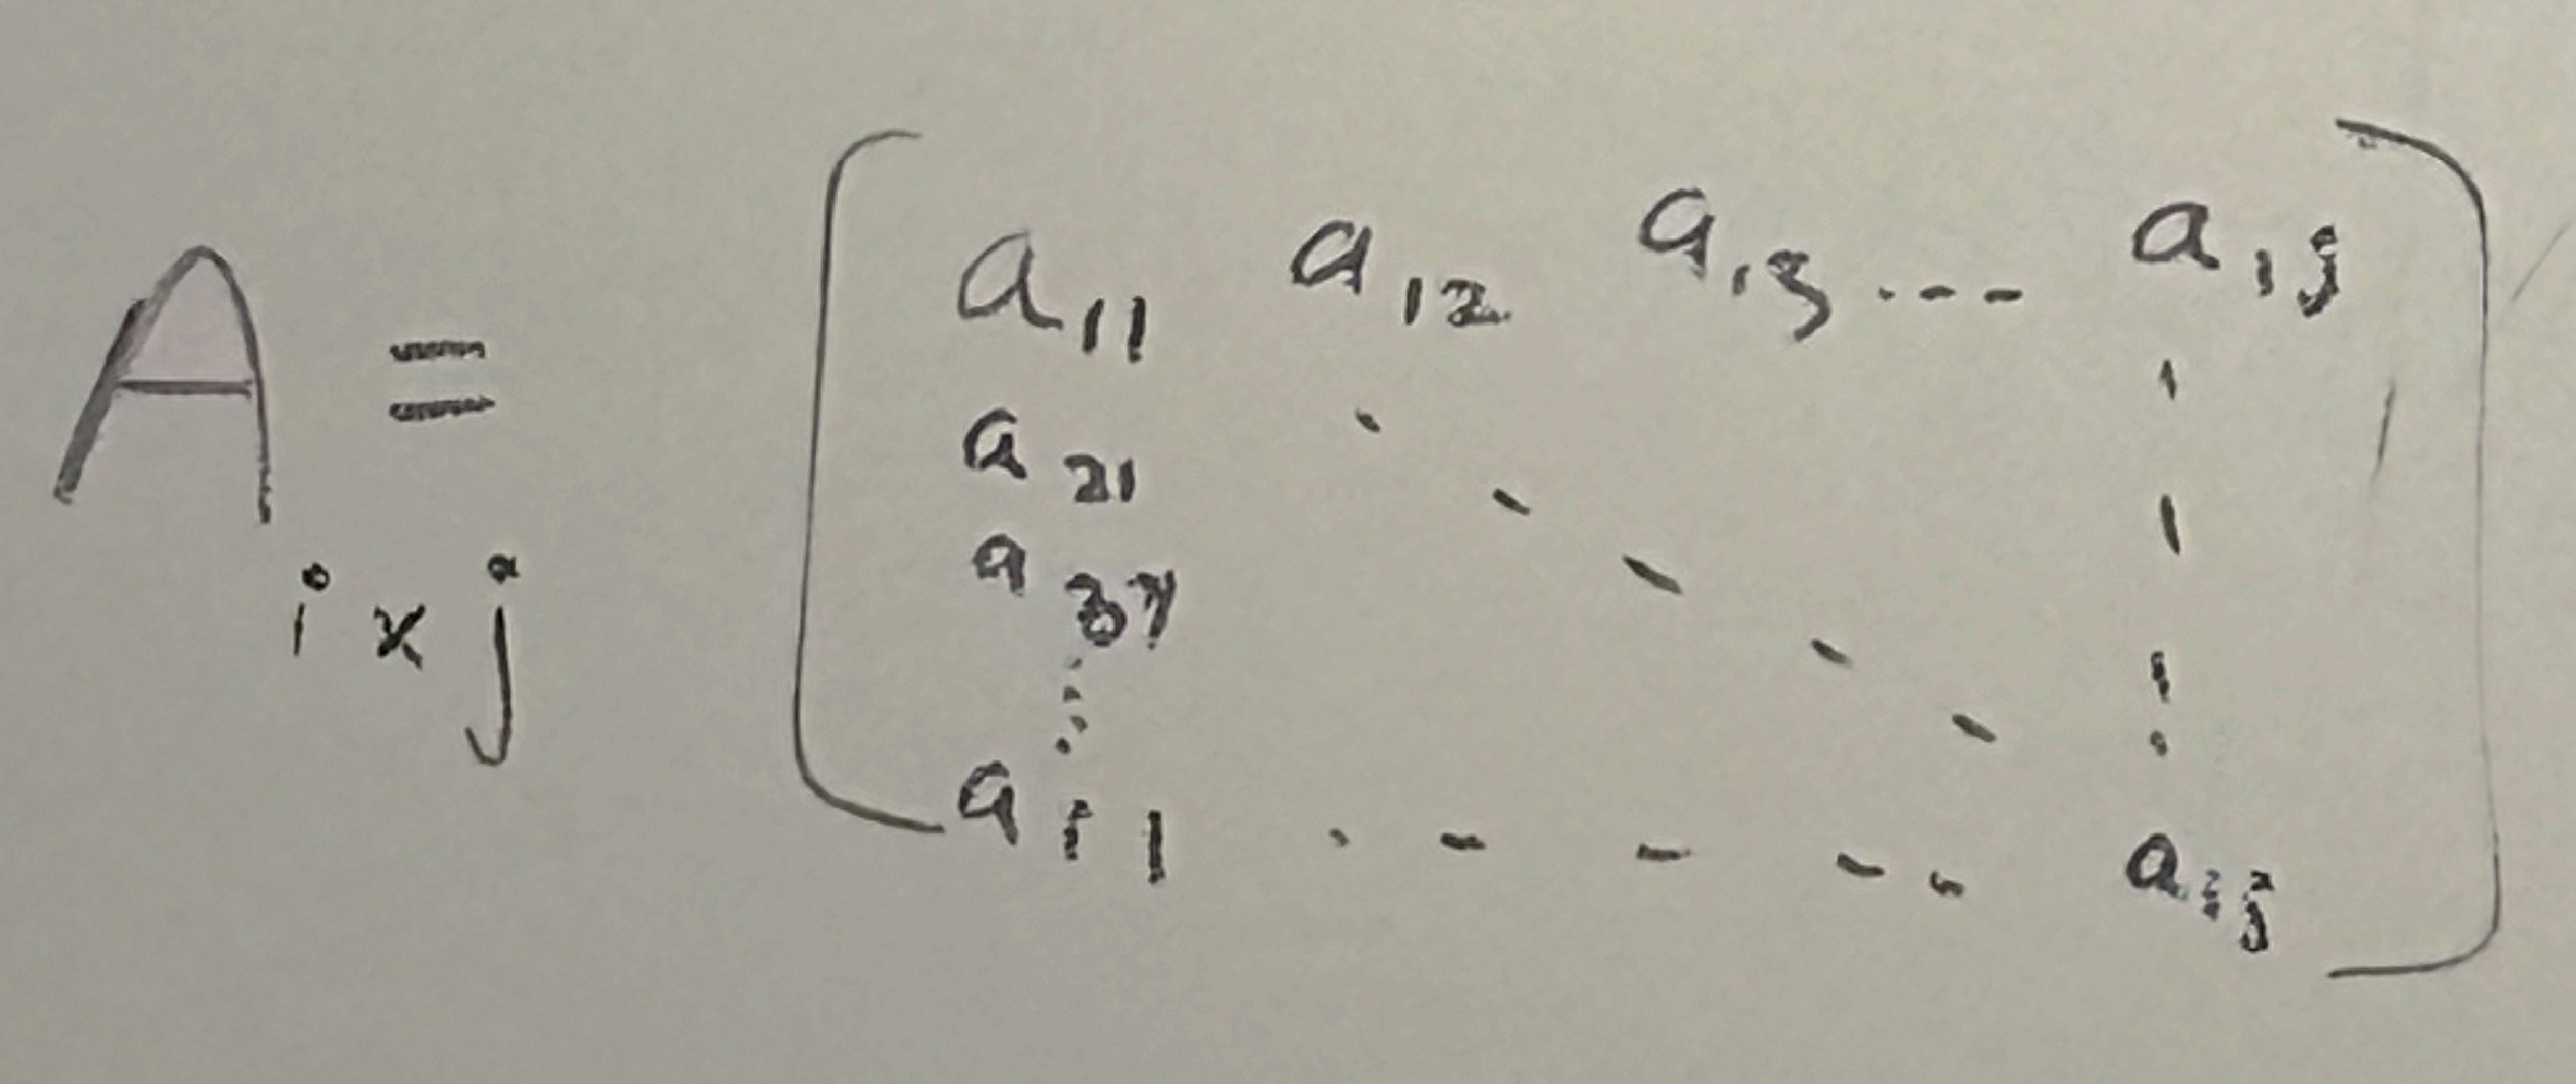
\includegraphics[width=0.5\linewidth]{matrix_terms.pdf}
    \label{fig:matrix_terms}
\end{figure}

One important thing to note is that systems may or may not have a solution - we will talk more about this later on. 

\subsubsection{Matrix operations}
In order to do any matrix operation, the matrices have to be conformable (i.e. their dimensions have to be suitable for the operation that we're doing). 

In order for two matrices to be equal to each other, every element must be equal to each other. In math:

\(A=C\) means that \(A_{ij}=C_{ij} \forall i,\forall j  \)

In order to add matrices, they need to have the same dimensions. When we add matrices, we add them element by element. The same applies for subtraction. 

Matrix multiplication is a little more complicated. We go over and down for each row. In order for a matrix to be comformable for multiplication, the number of columns of the first matrix must be equal to the number of rows of the second matrix. We also know that the resulting matrix will have the dimensions of the outer terms (\# of rows of the first matrix \( \times\) \# of columns of the second matrix).

\begin{figure}[H]
    \centering
    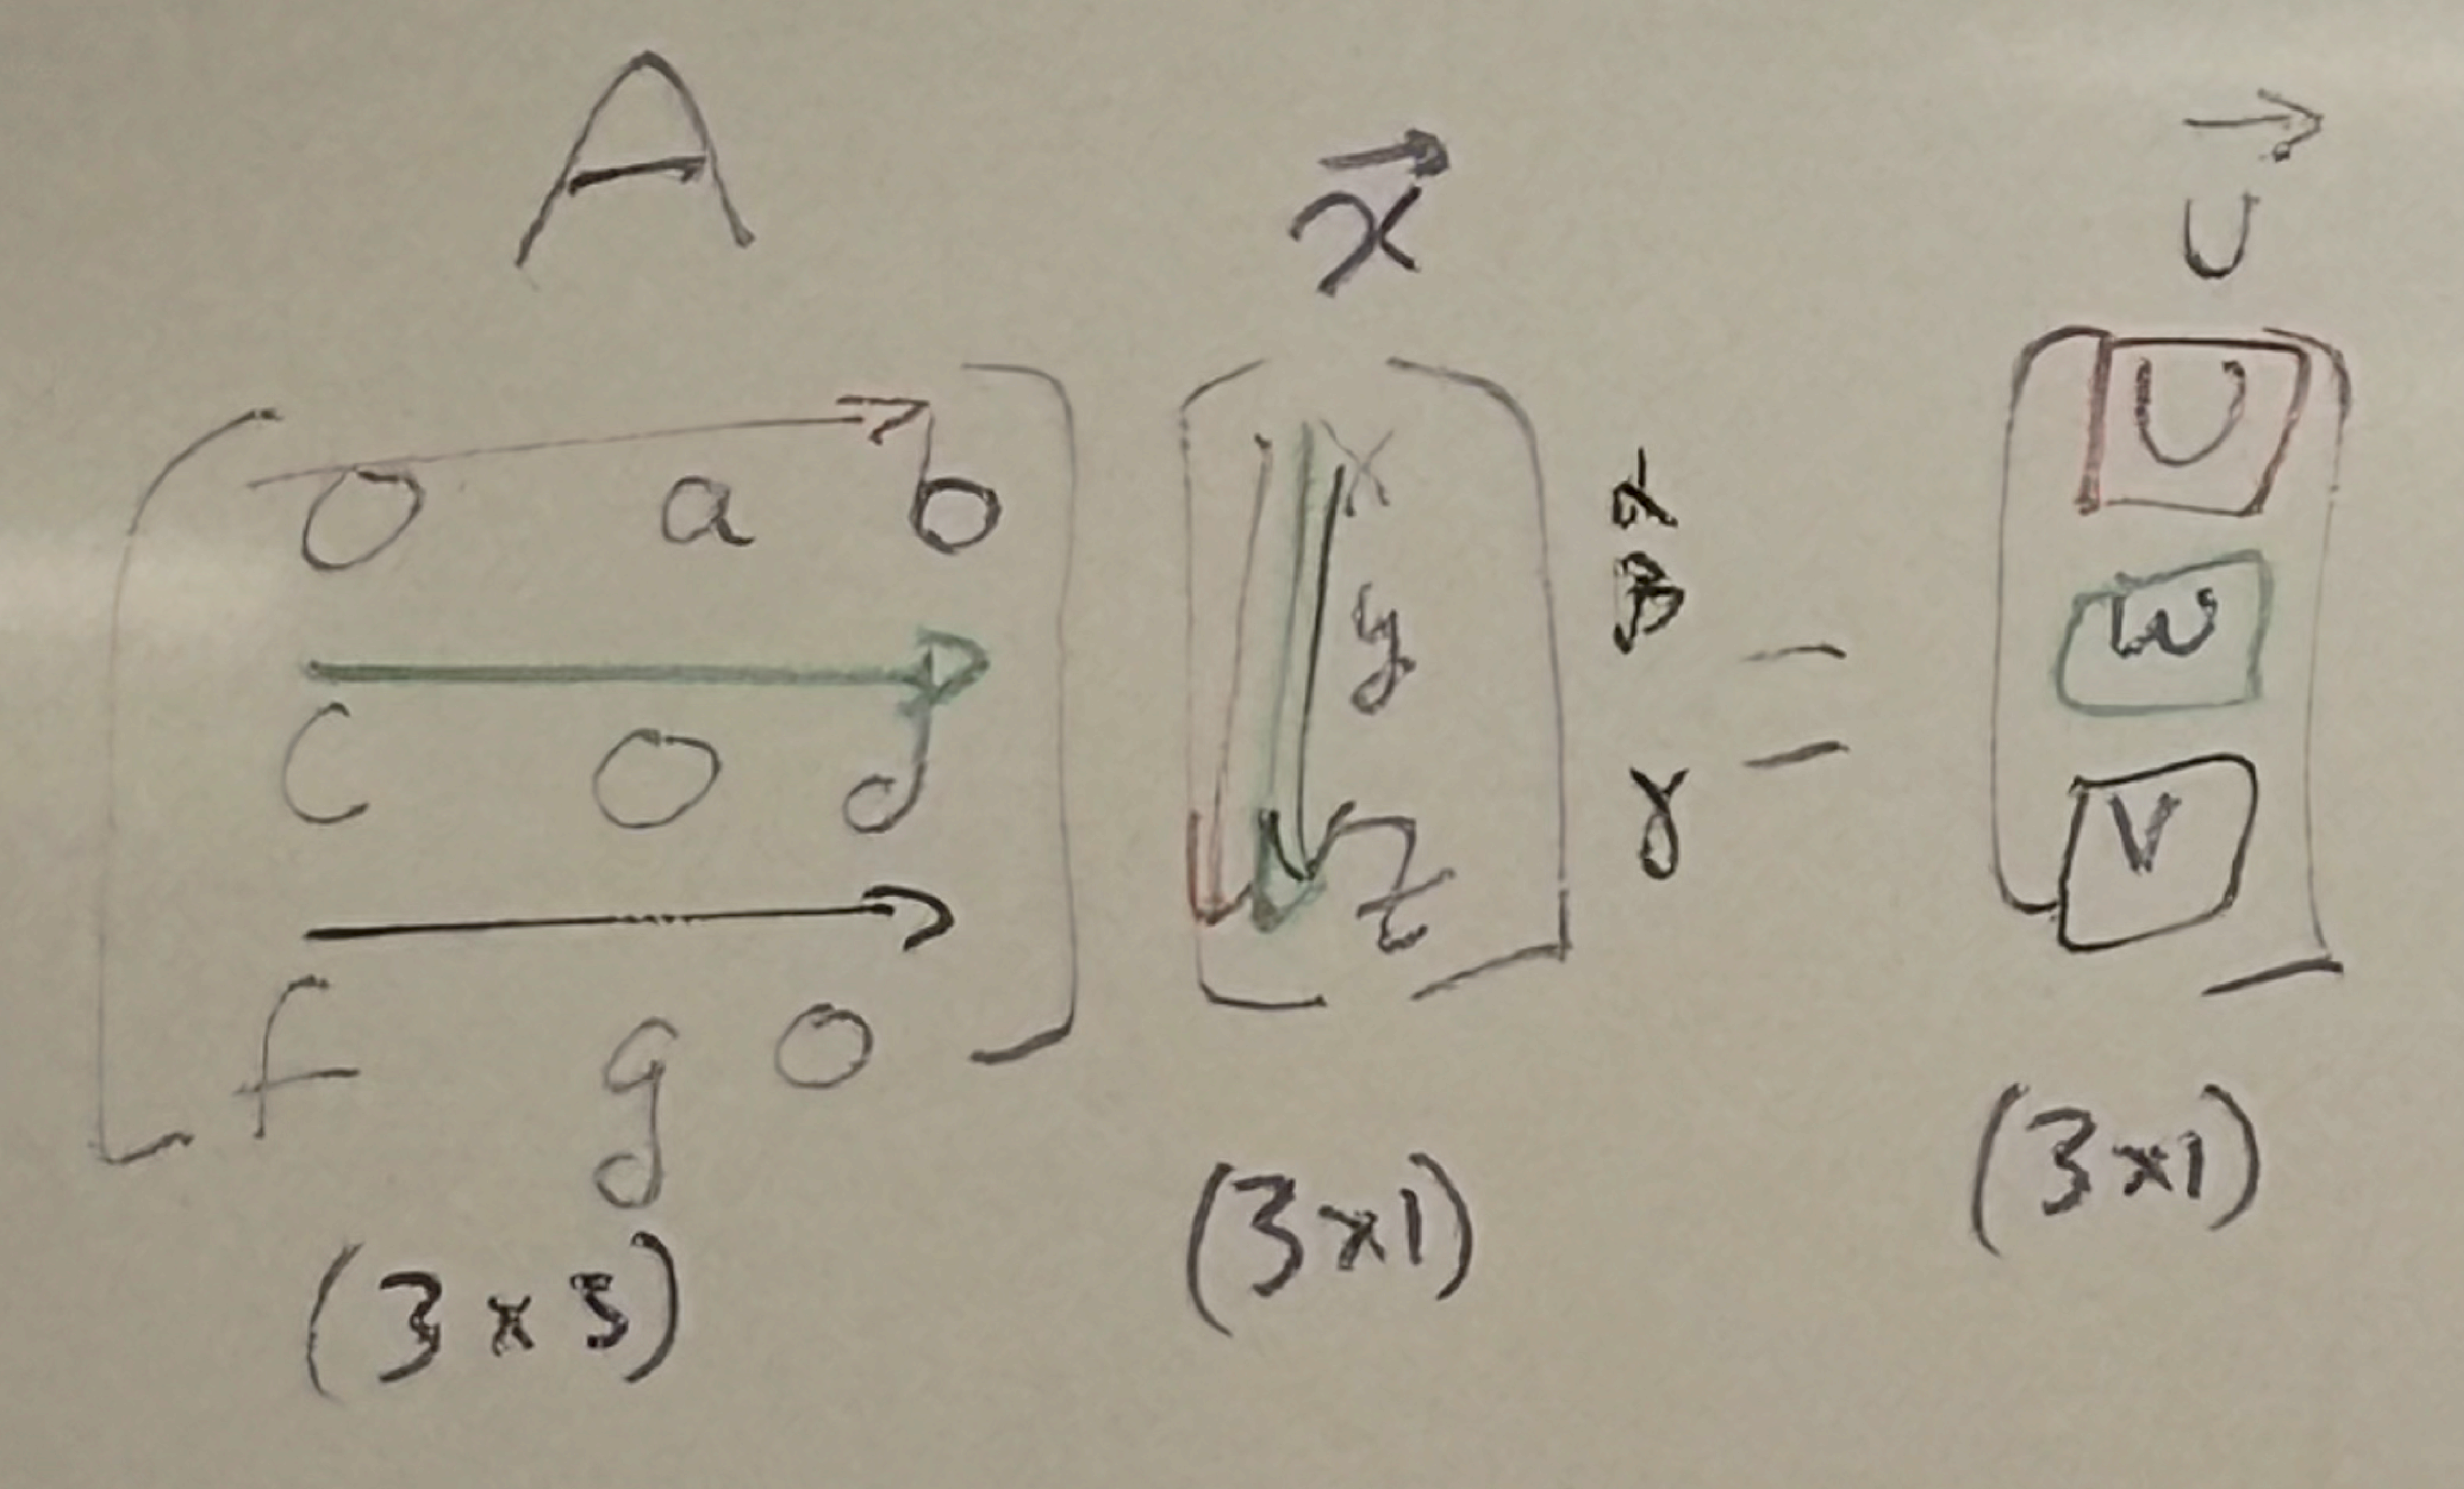
\includegraphics[width=0.5\linewidth]{matrix_multiplication.pdf}
    \label{fig:matrix_multiplication}
\end{figure}

\end{document}